\chapter{Simulaci\'{o}n Computacional}
Se estudia el cotransportador vSGLT mediante el servidor ANM de la universidad de Pittsburg \cite{Eyal2015}. 
\section{Modelo ANM de vSGLT}
\begin{figure}
 \centering
  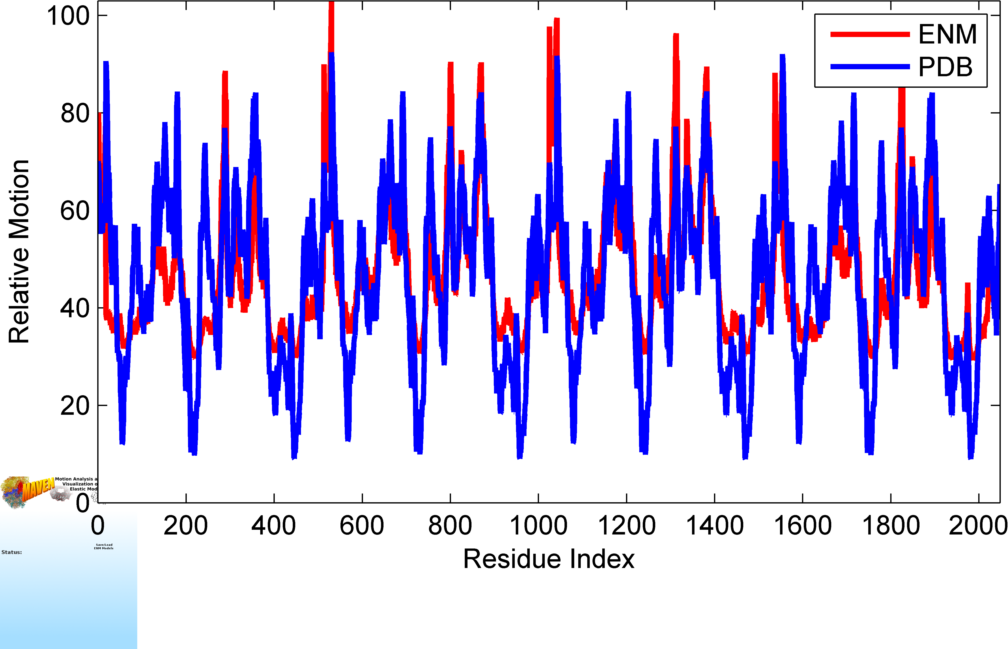
\includegraphics[scale=0.3]{./Kap4/ANM/Ca/BF_plot_100.png}
 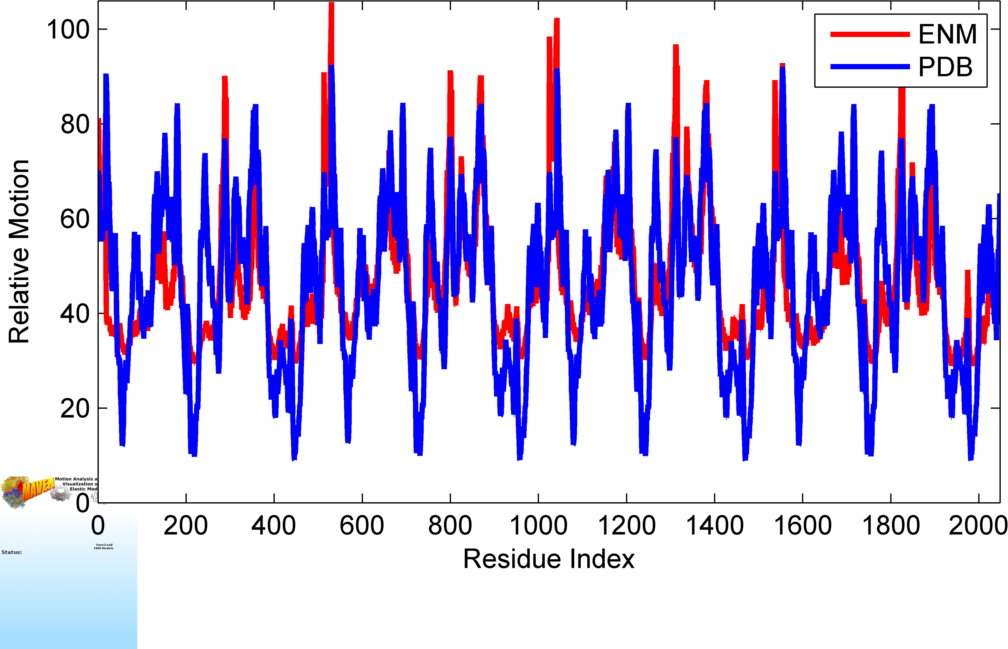
\includegraphics[scale=0.3]{./Kap4/ANM/Ca/BF_plot.png}
 \caption{ANM para $R_c=8\AA$ usando a) los primeros 100 modos. b) usando todos los modos}
\end{figure}
\begin{figure}
 \centering
  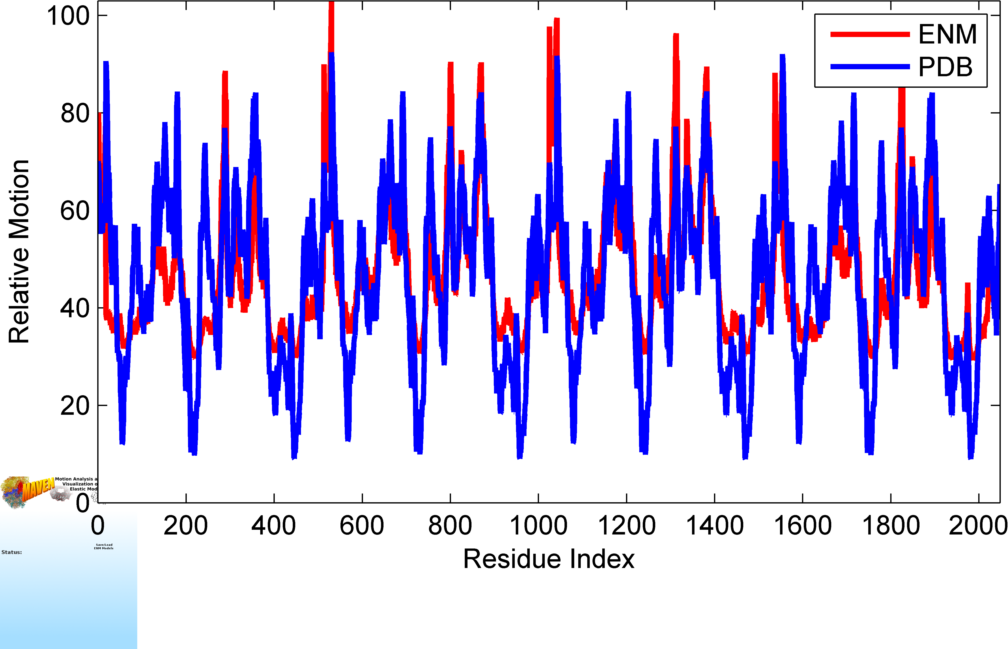
\includegraphics[scale=0.3]{./Kap4/ANM/Ca/BF_plot_100.png}
 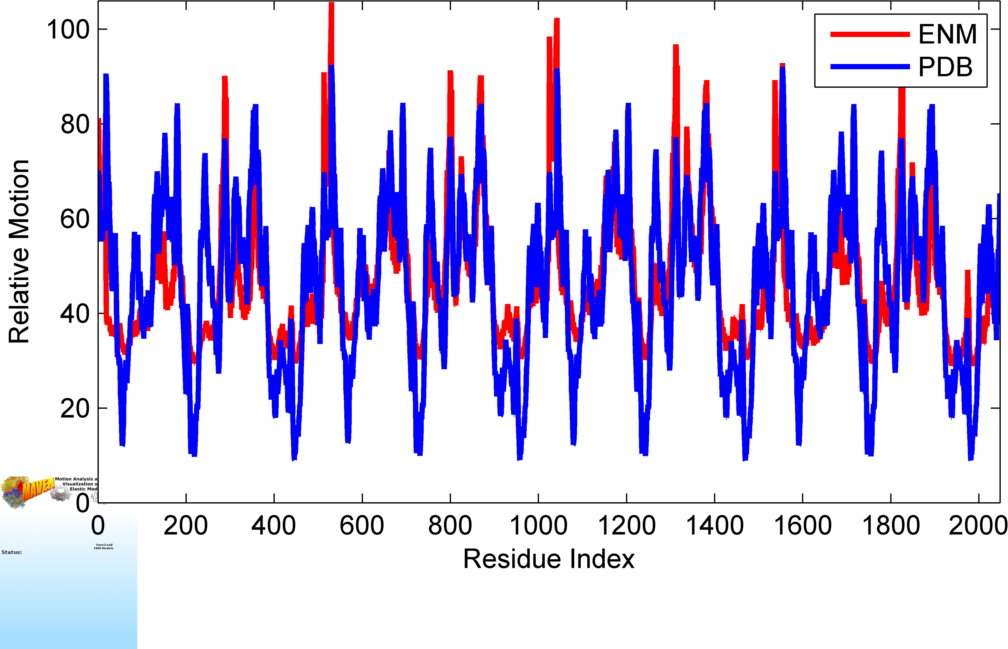
\includegraphics[scale=0.3]{./Kap4/ANM/Ca/BF_plot.png}
 \caption{ANM para $R_c=8\AA$ usando a) los primeros 100 modos. b) usando todos los modos}
\end{figure}
\section{Modelo GNM de vSGLT}

\section{Mutante K294A de vSGLT con C-$\alpha$}